% eEDM cancellation results
\begin{figure}[p]
    \centering
    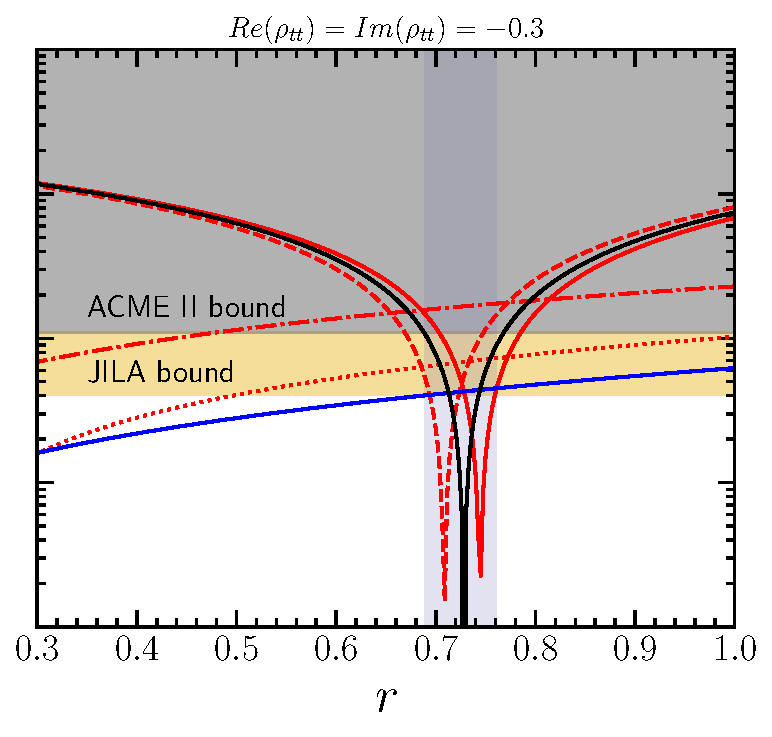
\includegraphics[width=6.95cm,height=5.55cm,angle=90]{fig2_3.pdf}\\
    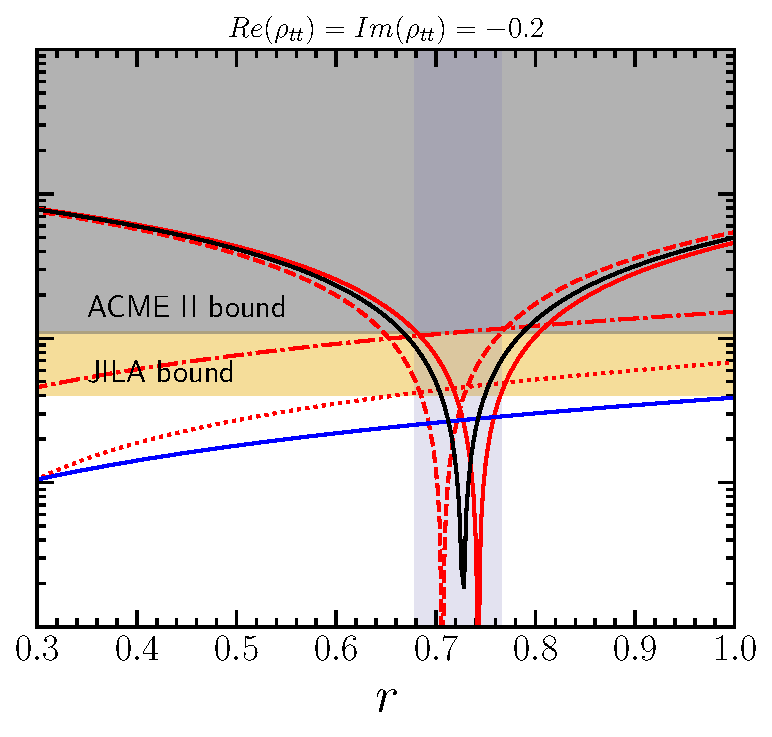
\includegraphics[width=6.95cm,height=5.55cm,angle=90]{fig2_2.pdf}\\
    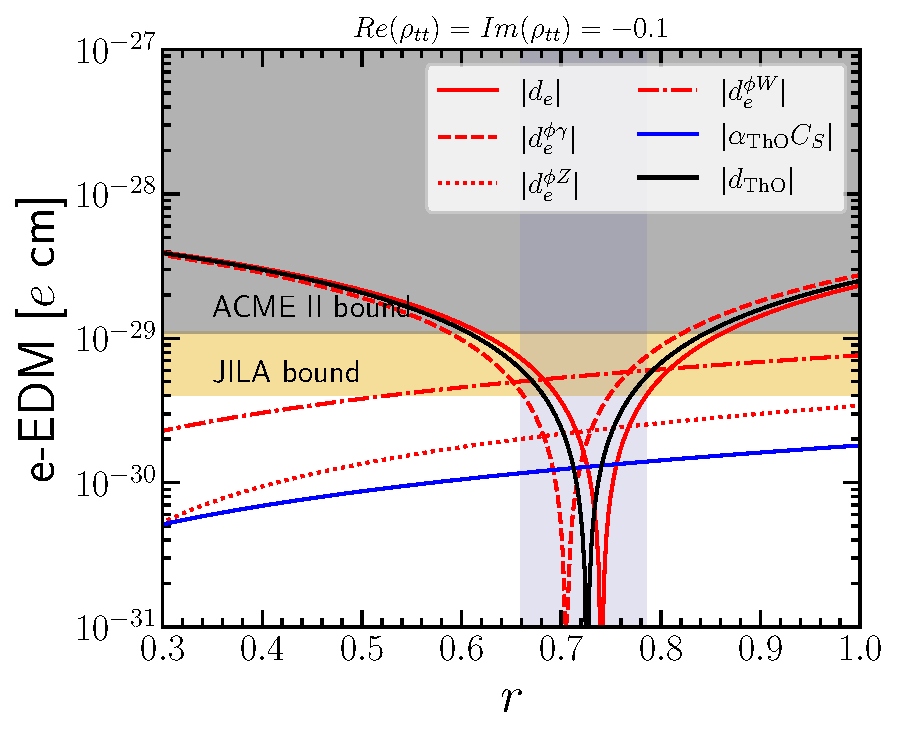
\includegraphics[width=7.95cm,height=5.55cm,angle=90]{fig2_1.pdf}
    \caption{eEDM v.s. \(r \) for a larger range of \(\rho_{tt} \) with ansatz~Eq.~\eqnref{eq:ansatz-extended}. (\(c_{\gamma} = 0.1, m_{H, A, H^+} = 500\,\mathrm{GeV} \))}
    \label{fig:eEDM}
\end{figure}

% muonEDM results
\begin{figure}[p]
    \centering
    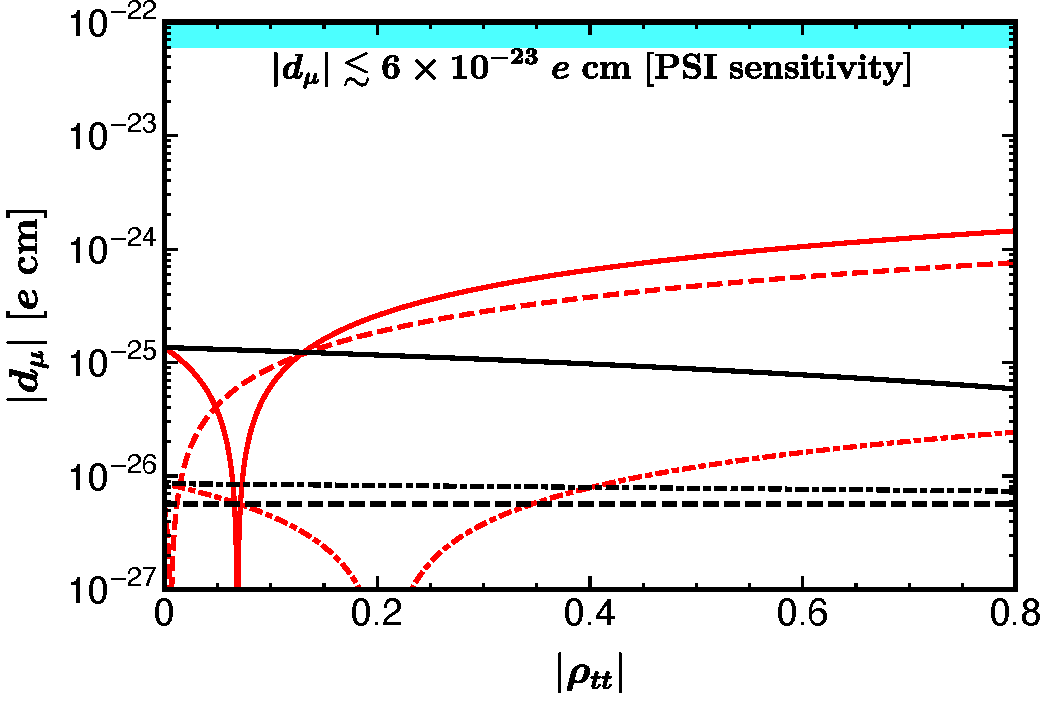
\includegraphics[width=0.7\textwidth]{muEDM.pdf}
    \caption{\(\mu \)EDM results.}
    \label{fig:muEDM}
\end{figure}

% tauEDM results
\begin{figure}[p]
    \centering
    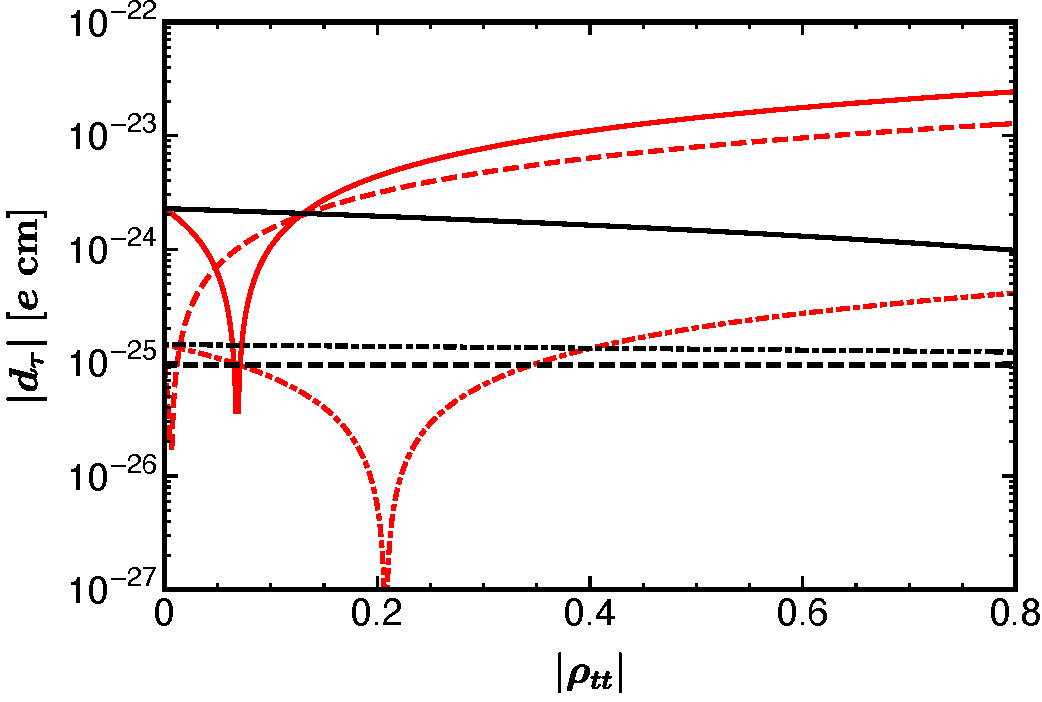
\includegraphics[width=0.7\textwidth]{tauEDM.pdf}
    \caption{\(\tau \)EDM results.}
    \label{fig:tauEDM}
\end{figure}